% File project.tex
%% Style files for ACL 2021
\documentclass[11pt,a4paper]{article}
\usepackage[hyperref]{acl2021}
\usepackage{times}
\usepackage{booktabs}
\usepackage{todonotes}
\usepackage{latexsym}
\usepackage{array,tabularx}
\renewcommand{\UrlFont}{\ttfamily\small}

% This is not strictly necessary, and may be commented out,
% but it will improve the layout of the manuscript,
% and will typically save some space.
\usepackage{microtype}

% Added by Yanlin
\usepackage{graphicx}
\usepackage{caption}
\usepackage{subcaption}
\usepackage{threeparttable}

\aclfinalcopy 

\newcommand\BibTeX{B\textsc{ib}\TeX}

\title{11-777 Report 1: Dataset Proposal and Analysis}

\author{
  Hao Wu\thanks{\hspace{4pt}Everyone Contributed Equally -- Alphabetical order} \hspace{2em} Jiayi Shen$^*$ \hspace{2em} Yanlin Feng$^*$ \hspace{2em} Yinghuan Zhang$^*$ \hspace{2em} Yuwei Wu$^*$\\
  \texttt{\{haowu3, jiayis2, yanlinf, yinghuan, yuweiwu\}@andrew.cmu.edu}
  }

\date{}

\begin{document}
\maketitle

\section{Problem Definition and Dataset Choice}
% If you are choosing a dataset not listed on the course website, this section should be long enough to justify that you are qualified for your choice.  This may mean a second page.

TextVQA \cite{Singh_2019_CVPR} is a Visual Question Answering (VQA) dataset that requires reasoning about text in images. In this section, we present a preliminary analysis of the fundamental challenges in this dataset and propose several hypotheses that can help improve performance over the current state of the art.


\subsection{What phenomena or task does this dataset help address?}
This dataset helps address the task of VQA that requires reading and reasoning over the text in images. The task is commonly needed by the visually impaired users.
\subsection{What about this task is fundamentally multimodal?}
This task involves visual and text modalities. Solving this task requires the model to leverage both visual and text content. 
\subsection{Hypotheses}
We believe there are six places where cross-modal information can be used or improved.
  \begin{enumerate}
    \item Spatial information can be used in combination of visual and text features to help improve answer prediction.
    
    \item The original LoRRA model architecture can be improved by introducing a text generative model, which is able to predict multi-token answers by incorporating latent encoding of both visual and text features.
    
    \item OCR can become more robust to transformation (rotation, scaling, etc) with the help of transformation information inferred by object detection module. 
    \item There are several data augmentation mechanisms we can explore to enhance the model's multi-modal representation learning, including corruption of images and OCR tokens as well as spatial bias augmentation for the detection boxes.
    \item To better model the interaction between visual and text features, we have also come up with two training strategies for the VQA task: one is to train with masked answer tokens in OCR, and the other is to train with relevant image patches masked. 
    \item In addition to prediction accuracy, evaluation can also be conducted under the Average Normalized Levenshtein Similarity (ANLS) metric to avoid a harsh zero score when the prediction is slightly different from the ground truth. 
    
  \end{enumerate}
\subsection{Expertise}
We have the following expertise in the underlying modalities required by this task:
  \begin{enumerate}
      \item Hao Wu: Took CV in Fall 2021; experience in 3D vision.
      \item Jiayi Shen: Took Intro to Machine Learning in Fall 2021, and taking Intro to Deep Learning this semester.
      \item Yanlin Feng: Research experience in question answering, knowledge graph reasoning, graph neural networks and multilingual NLP.
      \item Yinghuan Zhang: Took Intro to Machine Learning and Intro to Deep Learning in Fall 2021.
      \item Yuwei Wu: Have conducted research in NLP areas, including question answering, dialog systems, representation learning and multi-modal machine learning.
  \end{enumerate}

\section{Dataset Analysis}
\subsection{Dataset properties}

TextVQA v0.5.1 contains 45,336 questions based on 28,408 images. 
\begin{enumerate}
	\item Training set contains 34,602 questions (103 MB) based on 21,953 images (6.6 GB) from OpenImages' training set. 
	\item Validation set contains 5,000 questions (16 MB) based on 3,166 images from OpenImages' training set. 
	\item Test set contains 5,734 questions (13 MB) based on 3,289 images (926 MB) from OpenImages' test set.

\end{enumerate}

\subsection{Compute Requirements}
  \begin{enumerate}
    \item Files: the upper bound of memory cost for the entire training set is about 6.6GB. We are able to fit it in our servers. 
    \item Baseline Models:
    \begin{enumerate}
        \item \textbf{LoRRA}: training modules include one LSTM and two attention modules, trained for 24000 iterations with a batch size of 128 on 8 GPUs (not specified in the paper);
        \item \textbf{M4C}: training modules include BERT-base and the last layer of the Faster R-CNN, together taking 10 hours on 4 Nvidia Tesla V100 GPUs of batch size 128;
        \item \textbf{SAM}: training modules include two BERT-Base models. It took 12 hours to train 100 epochs on 2 NVIDIA Titan XP GPUs with batch size 96; 
        \item \textbf{LayoutLM}: training modules include one BERT-large model. It requires about 12-16 GB GPU memories to train the model for 100 epochs with batch size 16.
    \end{enumerate}
  \end{enumerate}
  
\subsection{Modality analysis}
\subsubsection{Text Analysis}

To better understand the TextVQA dataset from the language perspective, we conduct an analysis on the questions and answers on all three data splits. TextVQA contains 45336 questions in total, of which 37912 are unique. Following the original paper, we visualize the distribution of question lengths on all three data splits in Figure \ref{subfig:qlength}. Since the TextVQA validation and test split are randomly sampled, the distribution is almost identical across data splits. The average question lengths in the three data splits are 7.18/7.21/7.11 respectively. As shown in Figure \ref{subfig:top10start}, more than 78\% of the questions in TextVQA are what-questions. We also show the 10 most frequent questions and their frequency in Figure \ref{subfig:top10q}. The distribution of the 10 most frequent answers is shown in Figure \ref{subfig:top10a}. It is worth noting that more than 600 questions are labeled as unanswerable while more than 400 questions are labeled as ``answering does not require reading text in the image''. Other answers in TextVQA include various entity types like numbers, brands, cities, time, and people's names.

    
%%%%%%%%%%%%%%%%%%%%%%%%%%%%%%%%%%%%%%%%%%%%%%%%%%%%
\begin{figure*}[h]
  \centering
  \begin{subfigure}[b]{0.8\textwidth}
    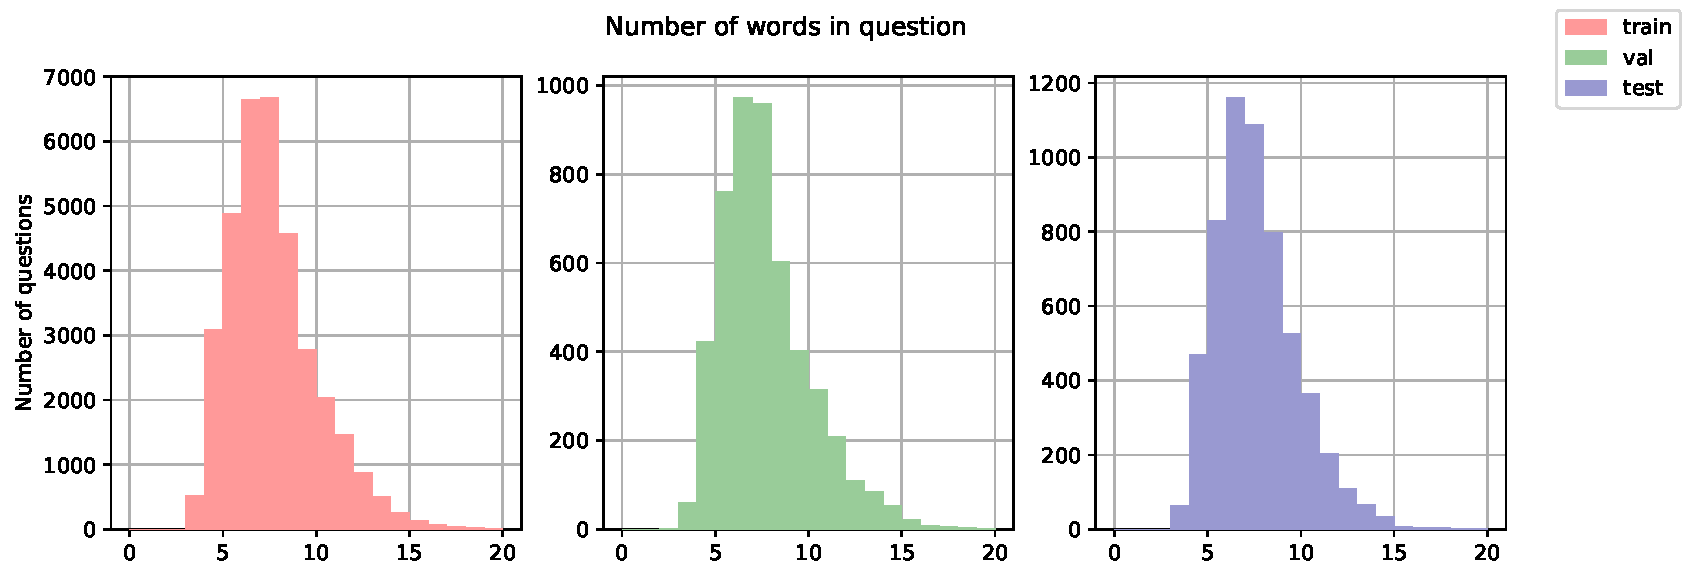
\includegraphics[width=\textwidth]{figures/qlength.pdf}
    \caption{}
    \label{subfig:qlength}
  \end{subfigure}
  
   \begin{subfigure}[b]{0.8\textwidth}
    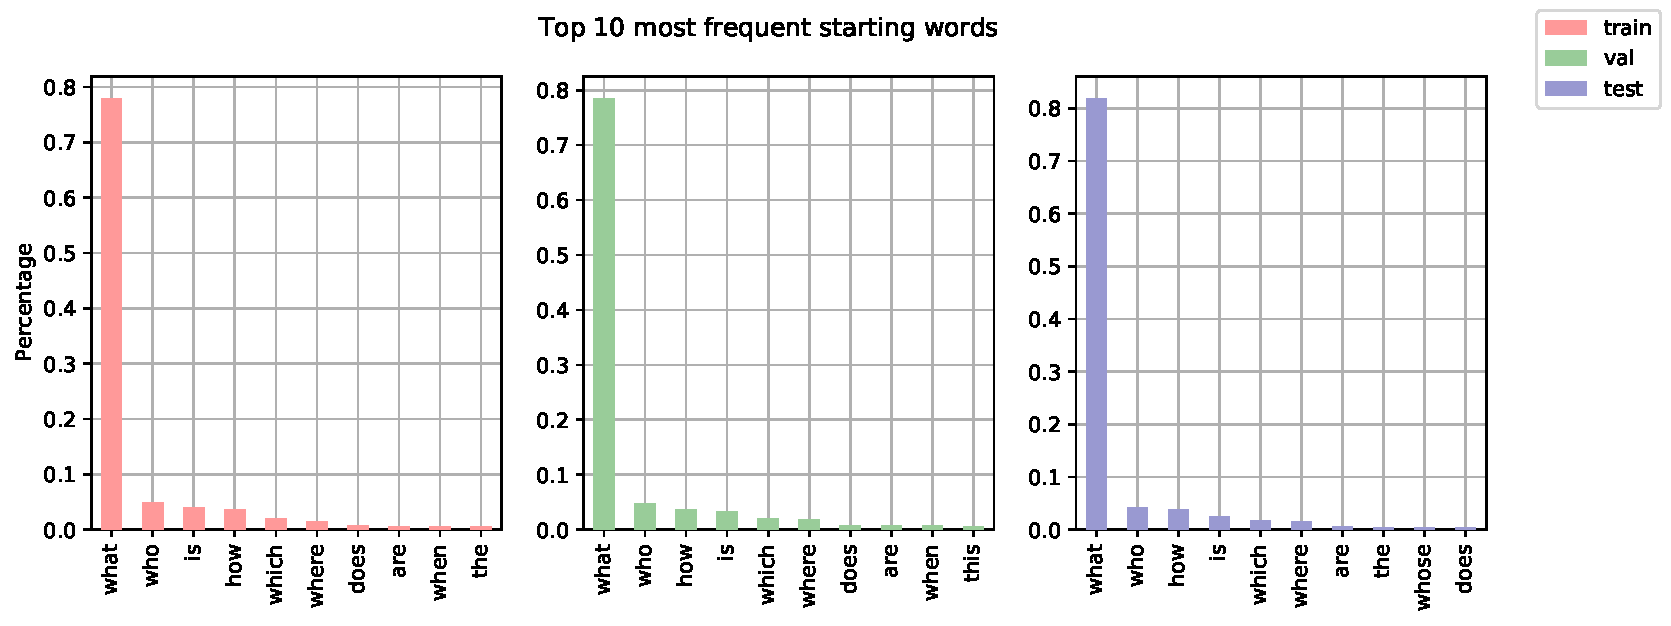
\includegraphics[width=\textwidth]{figures/top10start.pdf}
    \caption{}
    \label{subfig:top10start}
  \end{subfigure}
  
  \begin{subfigure}[b]{0.8\textwidth}
    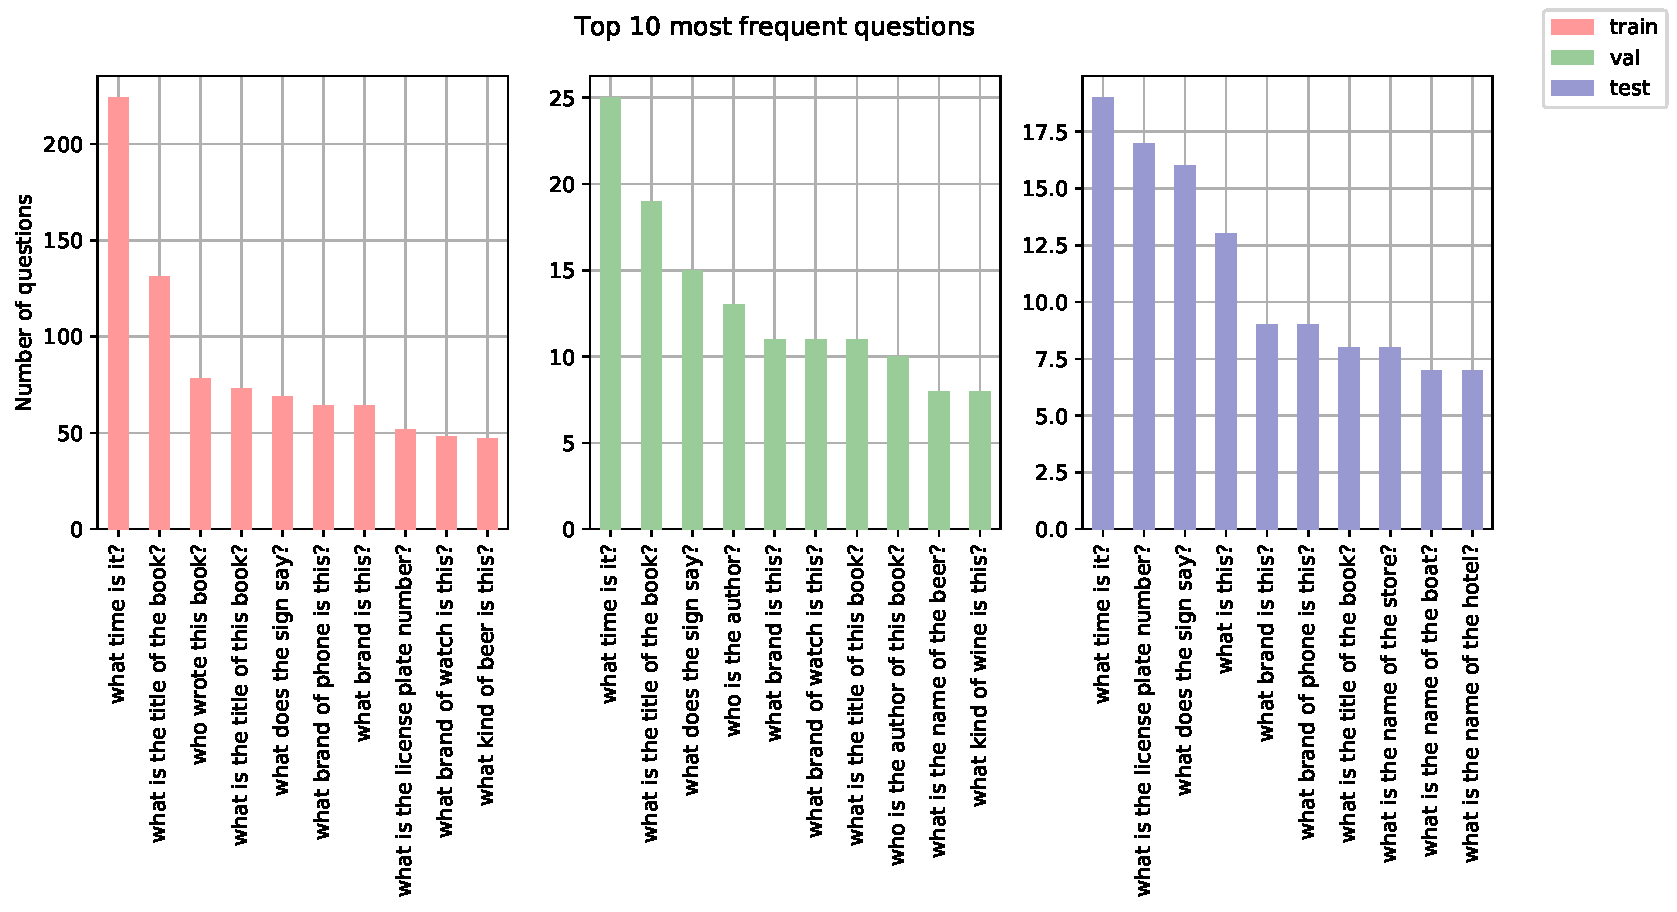
\includegraphics[width=\textwidth]{figures/top10q.pdf}
    \caption{}
    \label{subfig:top10q}
  \end{subfigure}
  
  \begin{subfigure}[b]{0.5\textwidth}
    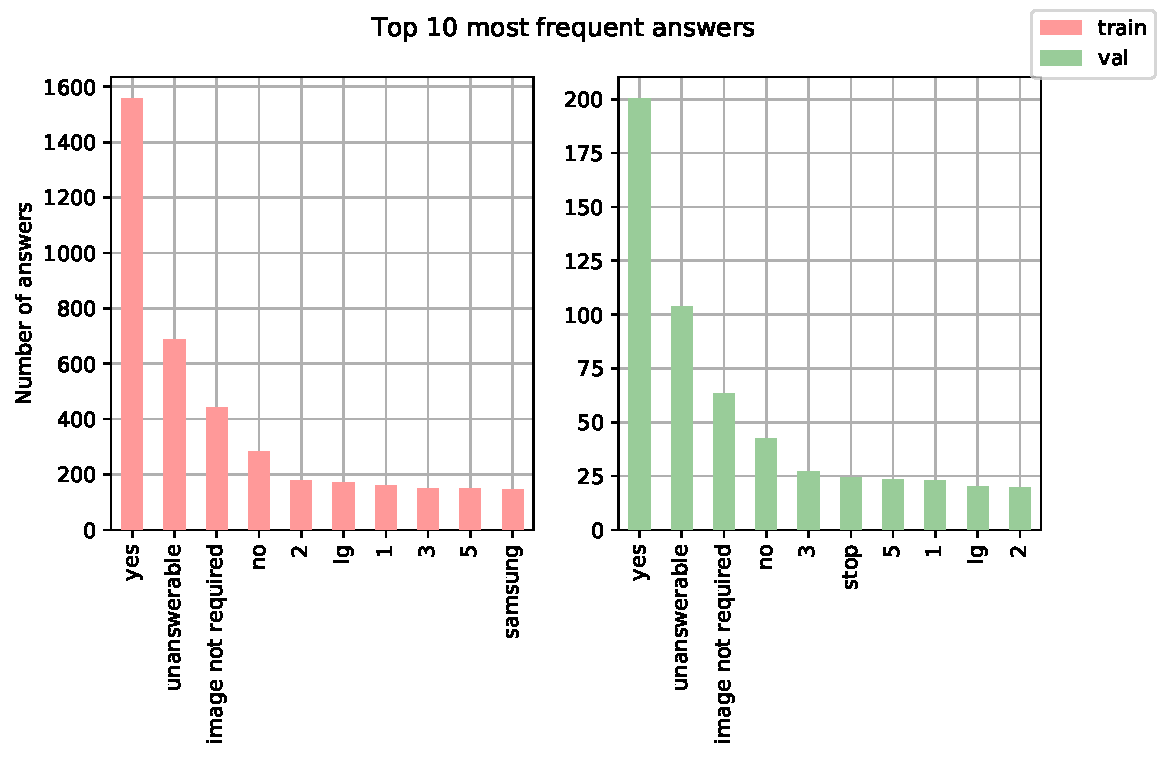
\includegraphics[width=\textwidth]{figures/top10a.pdf}
    \caption{}
    \label{subfig:top10a}
  \end{subfigure}

  \caption{Text statistics of the TextVQA dataset.}
  \label{fig:asdf}
\end{figure*}
%%%%%%%%%%%%%%%%%%%%%%%%%%%%%%%%%%%%%%%%%%%%%%%%%%%%

\subsubsection{Vision Data Analysis}

\begin{table}[h]
\caption{TextVQA dataset Rosetta OCR Error Analysis}
\label{ocr_error_analysis}
    \begin{center}
        \begin{tabularx}{\linewidth}{c|X X X}
            \hline
            \textbf{Dataset} & Error Rate & Detection Error Rate & Token Error Rate \\\hline
            \textbf{Training} & 29.17\% & 7.41\% & 23.50\% \\
            \textbf{Validation} & 40.55\% & 6.67\% & 31.58\% \\
            \textbf{Test} & 29.92\% & 15.35\% & 17.21\% \\
            \hline
            \textbf{Overall} & 32.05\% & 9.80\% & 24.67\% \\
            \hline
        \end{tabularx}
    \end{center}
\end{table}

We conduct exploratory analysis on vision data of TextVQA dataset, i.e., Rosetta OCR data following the original paper. To measure the error rate of OCR, we randomly sample 20 images from each of training set, validation set, and test set. \textit{Error Rate} measures the share of all incorrectly recognized tokens out of all detected boxes; \textit{Detection Error Rate} measures the share of OCR tokens generated from non-text boxes out of all detected boxes; and \textit{Token Error Rate} measures the recognition error rate among the detected boxes that do contain text, as shown in Table \ref{ocr_error_analysis}.

Moreover, the average numbers of objects and OCR tokens detected in each image are examined and presented in the Table \ref{obj_ocr_analysis}. It is worth noting that only 2897 out of 3289 images in the testing dataset are present in OpenImages' v0.6 dataset, which should contain all the image data according to the TextVQA web page.


\begin{table}[h]
\caption{Exploratory Analysis on Object \& OCR Tokens Detection }
\label{obj_ocr_analysis}
    \begin{center}
        \begin{tabularx}{\linewidth}{c|X X}
            \hline
            \textbf{Dataset} & Avg objects detected & Avg OCR tokens \\\hline
            \textbf{Training} & 5.04 & 12.45 \\
            \textbf{Validation} & 5.31 & 12.89 \\
            \textbf{Test} & 9.14$^1$ & 9.60 \\
            \hline
        \end{tabularx}
    \end{center}
    \begin{tablenotes}
        \item $^1$ Only 2897 out of 3289 testing images are present in OpenImages' v0.6 dataset
  \end{tablenotes}
\end{table}

By glancing over the data with OCR visualization, we conclude several troublesome problems of the Rosetta OCR data:
  \begin{enumerate}
    \item OCR tokens are designed to provide the model with answer candidates. A high \textit{Detection Error Rate} provides the model with more confusing and meaningless answer candidates; a high \textit{Token Error Rate}, even when the model can "copy" the correct answer space, brings the final accuracy down due to the incorrect recognition.
    \item Rosetta OCR recognizes each detection box into one token, which possibly consists of several words. The combination of the word, even each recognized correctly, is useless for the question answering model.
  \end{enumerate}
 
We present several typical errors in the model answering related to OCR data in Figure \ref{fig:ocr}. Specifically, Fig \ref{fig:incorrect_recognition} shows an image where correct answer can be "copied" from the OCR token, however, the OCR token is recognized incorrectly; Fig \ref{fig:multi_tokens_needed} detects and recognizes correctly, but multi tokens should be combined together as the answer; Fig \ref{fig:not_detected} has an answer that can be "copied" from the OCR token as well, whereas the answer is not detected by OCR model; Fig \ref{fig:partially_covered} is not answered correctly because the answer token is partially covered and OCR model is not able to complete it; Fig \ref{fig:ocr_not_helpful} has partial answer token correctly detected and recognized, however, the OCR is not helpful to obtain the rest part of the answer.

\begin{figure*}
\centering

\begin{subfigure}[b]{.4\textwidth}
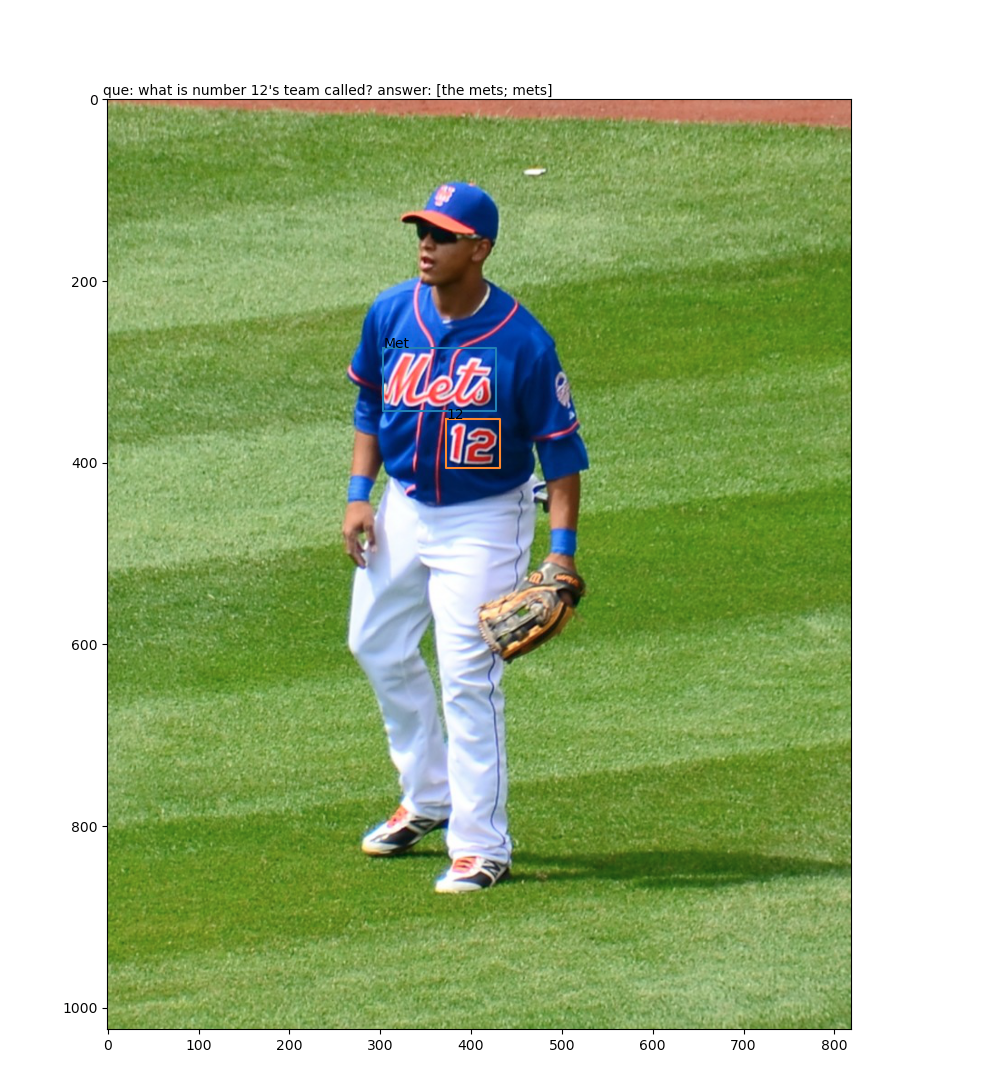
\includegraphics[width=\linewidth]{figures/incorrect_recognition.png}
\caption{Incorrect Recognition}\label{fig:incorrect_recognition}
\end{subfigure}
\begin{subfigure}[b]{.4\textwidth}
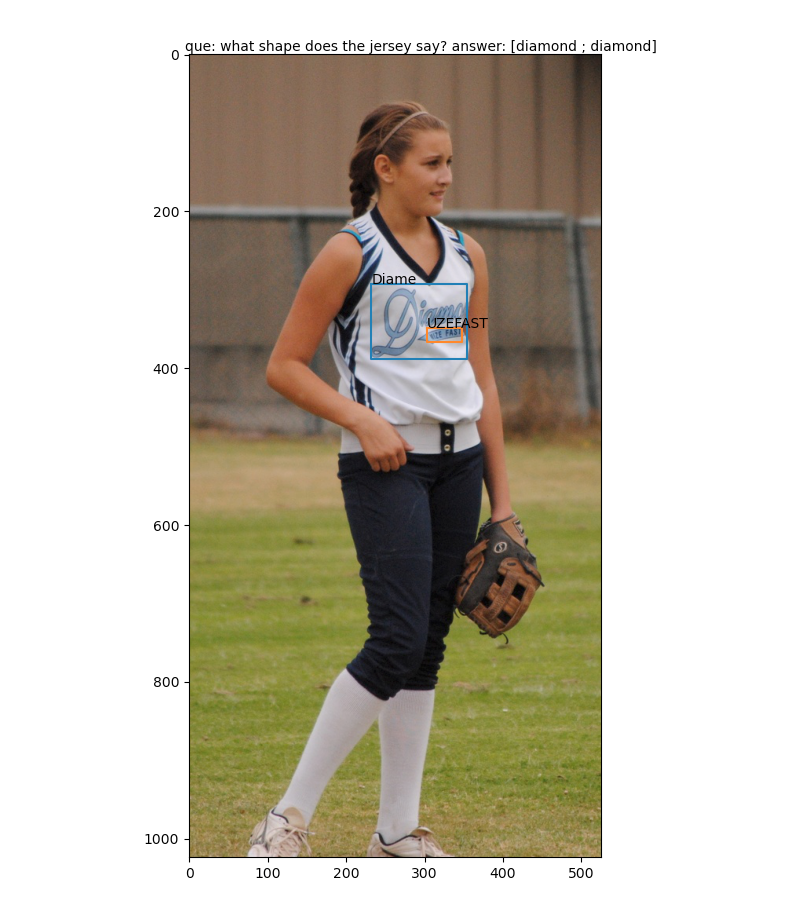
\includegraphics[width=\textwidth]{figures/partially_covered.png}
\caption{Text Partially Covered}\label{fig:partially_covered}
\end{subfigure}
\begin{subfigure}[b]{.33\textwidth}
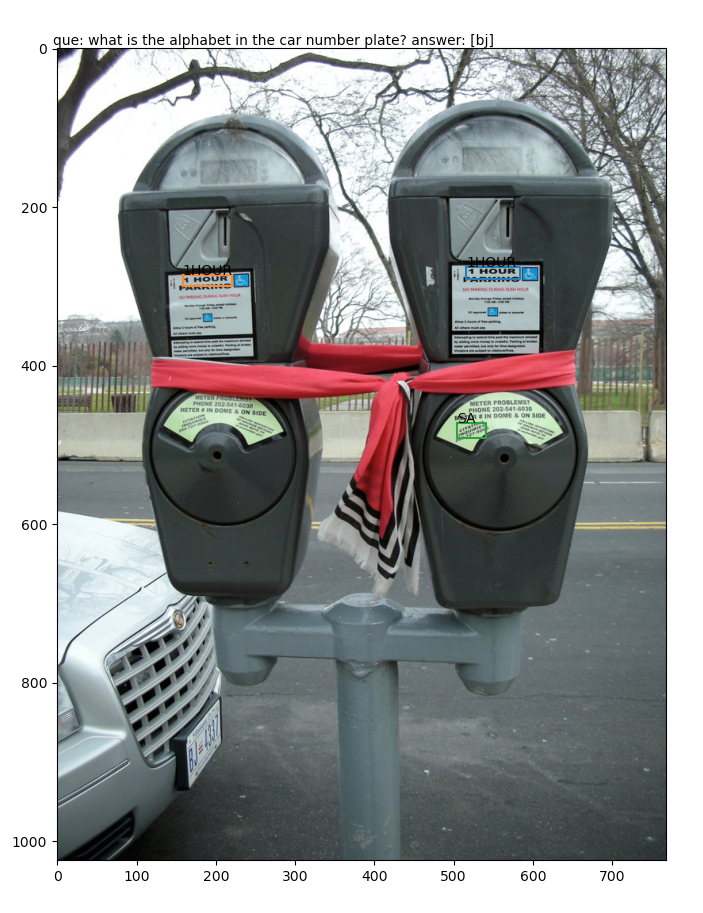
\includegraphics[width=\textwidth]{figures/not_detected.png}
\caption{Answer Not Detected}\label{fig:not_detected}
\end{subfigure}
\begin{subfigure}[b]{.5\textwidth}
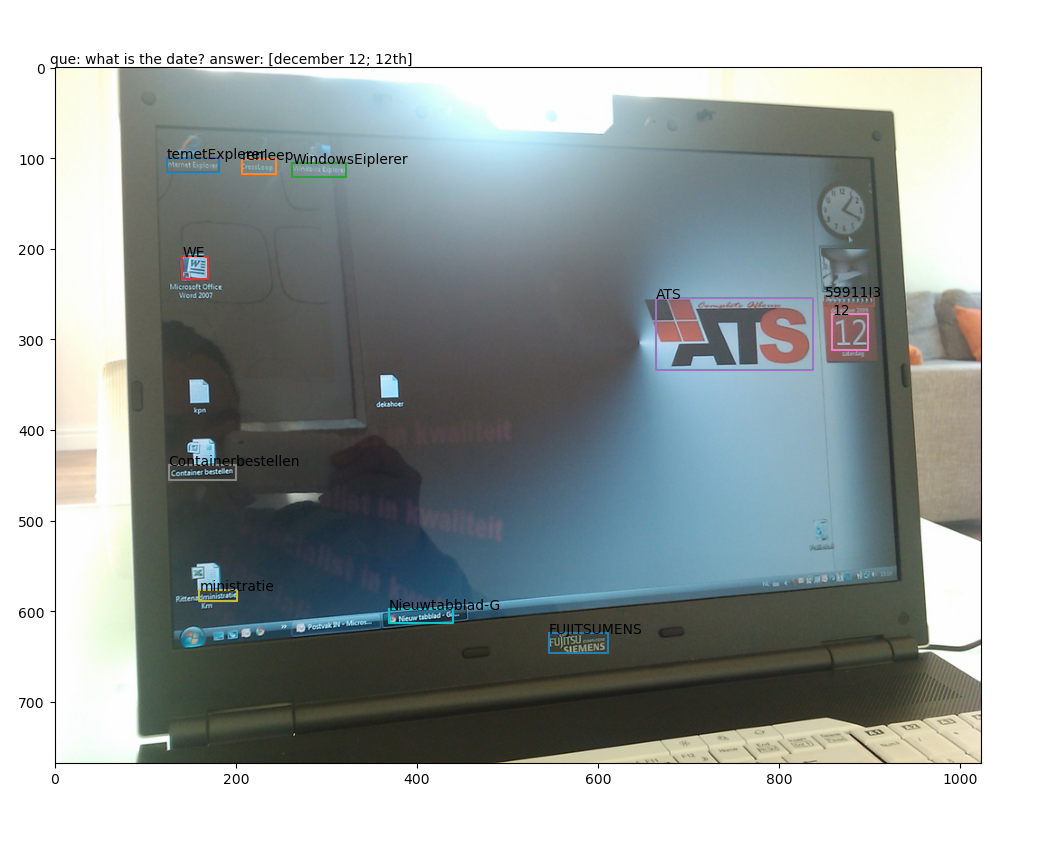
\includegraphics[width=\textwidth]{figures/ocr_not_helpful.png}
\caption{OCR Not Helpful}\label{fig:ocr_not_helpful}
\end{subfigure}
\begin{subfigure}[b]{.5\textwidth}
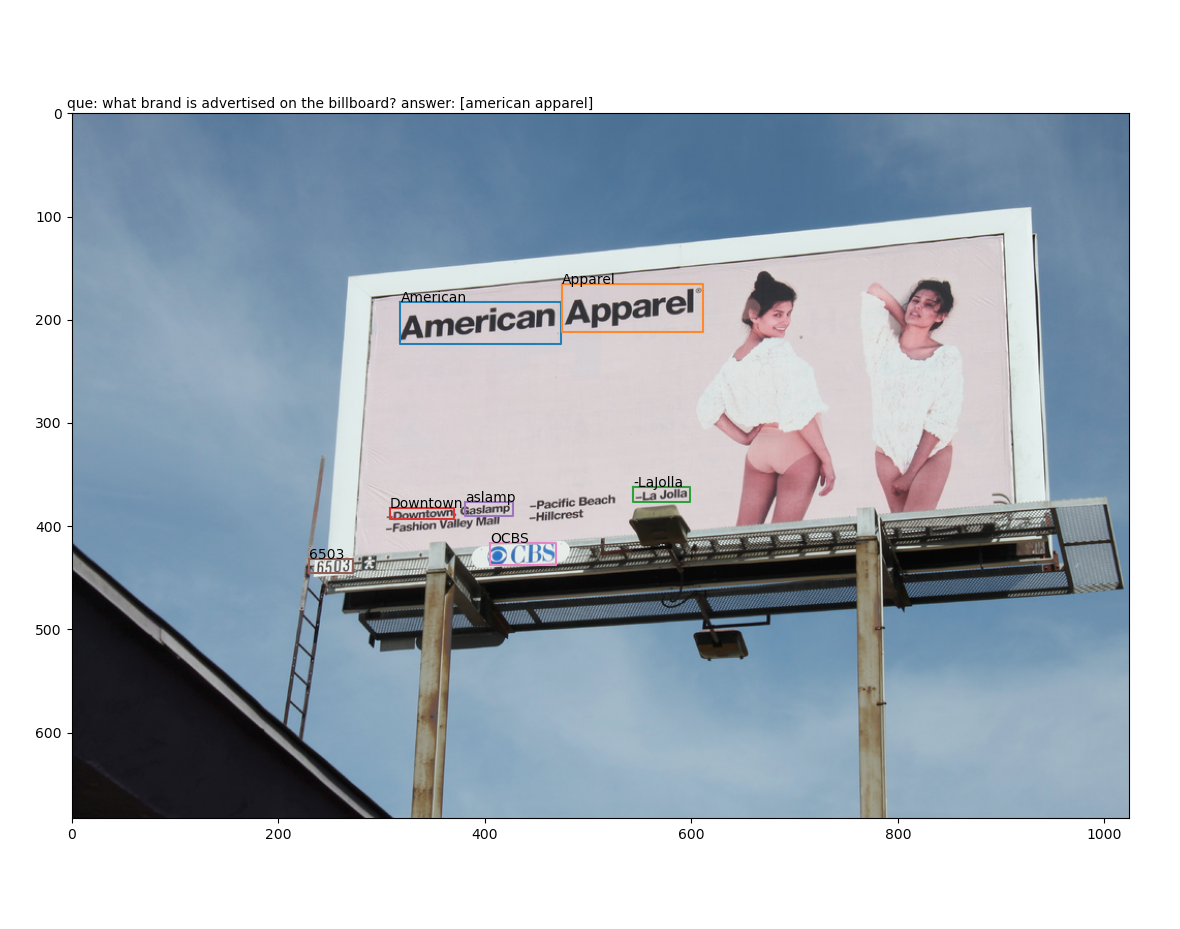
\includegraphics[width=\textwidth]{figures/multi_tokens_needed.png}
\caption{Need Multi Tokens}\label{fig:multi_tokens_needed}
\end{subfigure}

\caption{Typical errors related to OCR data.}
\label{fig:ocr}
\end{figure*}
  

\subsection{Metrics}
\begin{enumerate}
    \item Accuracy: the accuracy score between predicted answers and ground truth labels.
    \item Average Normalized Levenshtein Similarity (ANLS): the accuracy metric awards a zero score even when the prediction is only a little different from the target answer. Since no OCR is perfect, \citet{mathew2021docvqa} proposed the metric called ANLS for DocVQA task. Motivated by their work, we would also like to include this metric in our evaluation.
    
\end{enumerate}

\subsection{Baselines}
\begin{enumerate}
	\item \citet{Singh_2019_CVPR} introduced TextVQA dataset and the Look, Read, Reason \& Answer (\textbf{LoRRA}) architecture, which is based on a combination of visual detection and OCR module.
	\item \citet{hu2020iterative} proposed model \textbf{M4C} for the TextVQA task based on a multimodal transformer architecture accompanied by a rich representation for text in images.
	\item \citet{kant2020spatially} proposed model \textbf{SAM} with a novel spatially aware self-attention layer such that each visual entity only looks at neighboring entities defined by a spatial graph. Further, each head in the multi-head self-attention layer focuses on a different subset of relations.
	\item \citet{xu2020layoutlm} proposed \textbf{LayoutLM} for document image understanding, which jointly models the interactions between text and layout information and further leverages the image features through two pretraining tasks: masked visual language model and multi-label document classification.
	\item \citet{xu2021layoutlmv2} proposed \textbf{LayoutLM 2.0}, which is an extension of \textbf{LayoutLM} with two auxiliary pretraining tasks, namely Text-Image Alignment and Text-Image Matching. These two tasks help models to learn the correspondence between the document image and its textual content. The resulting model achieved the second place on the DocVQA dataset.
\end{enumerate}


\section{Team member contributions}
\paragraph{Hao Wu} contributed to the hypothesis proposal, exploratory data analysis on object and OCR token detection in images, and baseline summary.

\paragraph{Jiayi Shen} contributed to the text analysis and hypothesis ideas.

\paragraph{Yanlin Feng} contributed to the text analysis, baseline summary, and hypothesis ideas.

\paragraph{Yinghuan Zhang} contributed to the OCR error analysis, typical errors related to OCR data, and hypothesis ideas.

\paragraph{Yuwei Wu} contributed to the OCR analysis, baseline summary, and hypothesis ideas.


\clearpage
% Please use 
\bibliographystyle{acl_natbib}
\bibliography{references}

%\appendix



\end{document}
